\tikzstyle{boxes}=[draw=black, rounded corners,very thick]
\begin{center}
{
%\fontfamily{roman}{\fontsize{10}{10}\selectfont

\begin{tikzpicture}[shorten >=1pt,draw=black!50, x = 1 in, y = 1 in,  node distance=20pt]
\draw[draw=none, use as bounding box](-0.05,-0.1) rectangle (3.295,2.85);
\node[anchor=north west,align = flush left, text width=10 cm] at (-0.5,2.85) {Different representations can have very different performance, particularly if they do not preserve notions of chemical similarity correctly:};

%\draw[help lines,step=0.82] (0,0) grid (3.3,4);


%\node [anchor=north,rotate=90] (train) at (0.001,0.4) {nearest train.};

%\node [anchor=north,rotate=90] (train) at (0.001,1.2) {Fe(II)};
%\node [anchor=north,rotate=90] (train) at (0.87,1.2) {Fe(II)};
%\node [anchor=north,rotate=90] (train) at (1.69,1.2) {Fe(II)};

\visible<2->{\node [orange]  (liex) at (1.6,1.2) {{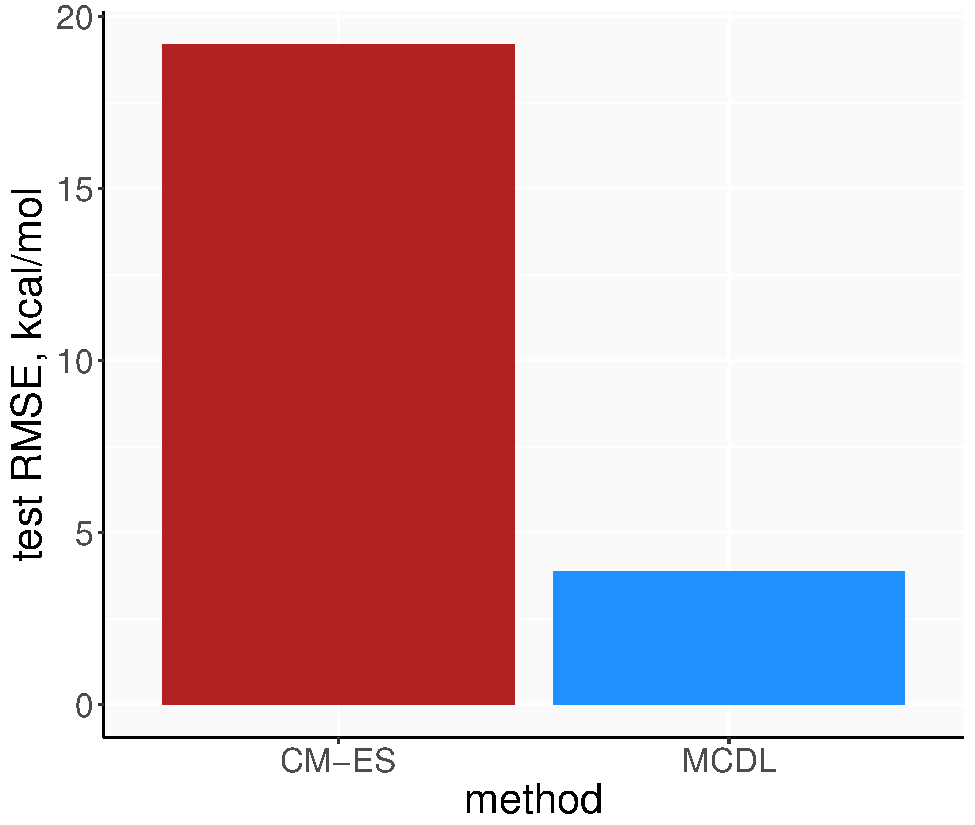
\includegraphics[width=6.0 cm]{representations/figures/error_comp}}};}

\visible<2->{\node[text width=10cm, align=flush left] at (2,0.01){\scriptsize{{Janet, J.P., and Kulik, H.J. \textit{Chem. Sci.}, 2017, 8, 5137-5152.}}};}
\end{tikzpicture}}
\end{center}


